\begin{center}\small
\begin{tabular}{llrrrr}\toprule
Variant & Engine & Budget & Mate / trials & Defense / trials & Overall\%\\\midrule
Enhanced & Alpha-beta & 0.1s & 4/6 & 4/6 & 66.7 \\
Enhanced & MCTS & 0.1s & 11/30 & 13/30 & 40.0 \\
Enhanced & Alpha-beta & 1s & 6/6 & 6/6 & 100.0 \\
Enhanced & MCTS & 1s & 0/30 & 3/30 & 5.0 \\
Enhanced & Alpha-beta & 5s & 6/6 & 6/6 & 100.0 \\
Enhanced & MCTS & 5s & 1/30 & 4/30 & 8.3 \\
Baseline & Alpha-beta & 0.1s & 0/6 & 3/6 & 25.0 \\
Baseline & MCTS & 0.1s & 2/30 & 14/30 & 26.7 \\
Baseline & Alpha-beta & 1s & 6/6 & 5/6 & 91.7 \\
Baseline & MCTS & 1s & 2/30 & 10/30 & 20.0 \\
\bottomrule\end{tabular}\end{center}
\subsubsection*{Search cost and MCTS stability}
\begin{center}\small\begin{tabular}{llrrrr}\toprule
Variant & Budget & AB depth & AB tactical nodes & MCTS simulations & Distinct moves\\\midrule
Enhanced & 0.1s & 2 & 315 & 33 & 3.92 \\
Enhanced & 1s & 3 & 2196.5 & 403.5 & 2.92 \\
Enhanced & 5s & 3.5 & 7205 & 1896 & 2.83 \\
Baseline & 0.1s & 2 & 0 & 14 & 4.58 \\
Baseline & 1s & 3 & 0 & 136.5 & 4.42 \\
\bottomrule\end{tabular}\end{center}
Depth, tactical nodes and simulations are medians. Distinct moves is the mean number
of different suggestions across five seeds per position; it ranges from 1 to 5.
These work counters measure different operations and must not be compared as equivalent nodes.
\subsubsection*{Wall-clock measurements}
\begin{center}\small\setlength{\tabcolsep}{4pt}\begin{tabular}{lrrrrr}\toprule
Variant & Budget & AB median (s) & MCTS median (s) & MCTS p95 (s) & Max overrun (ms)\\\midrule
Enhanced & 0.1s & 0.1001 & 0.1001 & 0.1003 & 0.762 \\
Enhanced & 1s & 0.6521 & 1.0000 & 1.0003 & 0.416 \\
Enhanced & 5s & 2.6608 & 5.0000 & 5.0001 & 0.274 \\
Baseline & 0.1s & 0.1001 & 0.1001 & 0.1004 & 0.526 \\
Baseline & 1s & 0.6397 & 1.0001 & 1.0004 & 0.702 \\
\bottomrule\end{tabular}\end{center}
Small overrun is measured and retained, not scored as a time-forfeit loss. Early proven mates can leave allocated time unused.
\subsubsection*{Color-swapped games}
\begin{center}\small\begin{tabular}{rrrrrrr}\toprule
Budget & Starts & Games & AB wins & Draws & AB losses & AB score\%\\\midrule
0.5s & 8 & 16 & 10 & 6 & 0 & 81.2 \\
5s & 2 & 4 & 4 & 0 & 0 & 100.0 \\
\bottomrule\end{tabular}\end{center}
For 0.5s, resampling the 8 paired starts 5,000 times gives a descriptive 95\% percentile interval [65.6\%, 93.8\%] for Alpha-beta's score.
This resampling keeps both colors together and uses seed 2352344. It reflects
variation among the selected starts, not a representative chess population.
No interval is reported for the two-start 5s subset: it is too small to support a useful precision claim.
\begin{figure}[ht]\centering
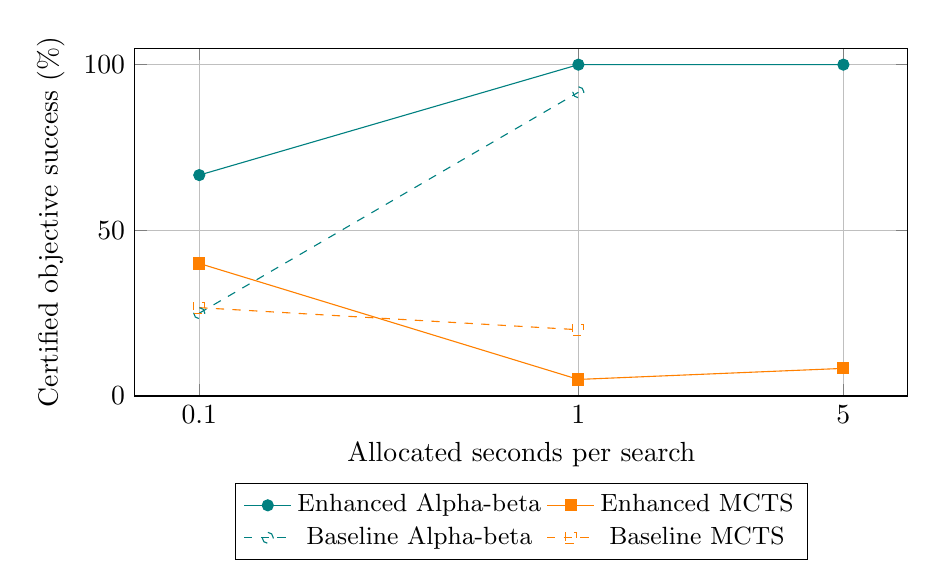
\begin{tikzpicture}\begin{axis}[width=.94\textwidth,height=6cm,xmode=log,
xlabel={Allocated seconds per search},ylabel={Certified objective success (\%)},
xtick={.1,1,5},xticklabels={0.1,1,5},ymin=0,ymax=105,grid=major,
legend style={at={(.5,-.25)},anchor=north,legend columns=2,font=\small}]
\addplot[teal,mark=*] coordinates {(0.1,66.667) (1.0,100.000) (5.0,100.000)};
\addlegendentry{Enhanced Alpha-beta}
\addplot[orange,mark=square*] coordinates {(0.1,40.000) (1.0,5.000) (5.0,8.333)};
\addlegendentry{Enhanced MCTS}
\addplot[teal,dashed,mark=o] coordinates {(0.1,25.000) (1.0,91.667)};
\addlegendentry{Baseline Alpha-beta}
\addplot[orange,dashed,mark=square] coordinates {(0.1,26.667) (1.0,20.000)};
\addlegendentry{Baseline MCTS}
\end{axis}\end{tikzpicture}
\caption{Success on the fixed certified corpus, combining attack and defense objectives. Baseline was tested at 0.1 and 1 seconds only. Lines connect measured budgets and do not predict intermediate performance.}\end{figure}
